
\section{Partie 2.a : Étude de l'architecture DNN DiffWave}
\label{sec:diffwave}

\subsection{Présentation générale de DiffWave}

DiffWave (\textit{Diffusion Model for Audio Synthesis}) est un modèle
génératif basé sur les modèles probabilistes de diffusion, proposé par
Kong et al. en 2021. Il permet de générer des formes d'onde audio
(\textit{waveforms}) à partir de bruit gaussien, avec ou sans information
de conditionnement.

Contrairement aux modèles autorégressifs classiques, DiffWave adopte
une architecture non autorégressive fondée sur des convolutions
dilatées bidirectionnelles. La génération audio repose sur un processus
itératif de débruitage qui transforme progressivement un signal
initialement aléatoire en une forme d'onde structurée.

L'article original présente trois applications principales :
\begin{itemize}
    \item le \textbf{neural vocoding}, conditionné par un
    spectrogramme Mel ;
    \item la \textbf{génération conditionnelle par classe}
    (\textit{class-conditional generation}) ;
    \item la \textbf{génération audio inconditionnelle}
    (\textit{unconditional generation}).
\end{itemize}

\subsection{Architecture générale du modèle}

DiffWave apprend un réseau de neurones noté
$\epsilon_\theta(x_t,t)$, dont le rôle est de prédire le bruit
présent dans le signal à une étape donnée du processus de diffusion.

Le réseau reçoit principalement :
\begin{itemize}
    \item le signal audio bruité $x_t$ à l'étape $t$ ;
    \item l'indice temporel de diffusion $t$ ;
    \item une information de conditionnement éventuelle, selon
    l'application considérée.
\end{itemize}

Le réseau estime alors le bruit ajouté au signal. Cette estimation
est utilisée par le processus inverse pour calculer une version
moins bruitée du signal.

L'architecture repose sur plusieurs éléments :
\begin{itemize}
    \item une convolution initiale $1\times1$ ;
    \item un embedding représentant l'étape de diffusion ;
    \item une succession de couches résiduelles utilisant des
    convolutions dilatées bidirectionnelles ;
    \item des connexions de saut (\textit{skip connections}) ;
    \item des convolutions finales permettant de produire
    l'estimation du bruit.
\end{itemize}

La Figure~\ref{fig:diffwave_architecture} présente l'architecture
du réseau telle qu'elle est proposée dans l'article original.

\begin{figure}[htbp]
    \centering
    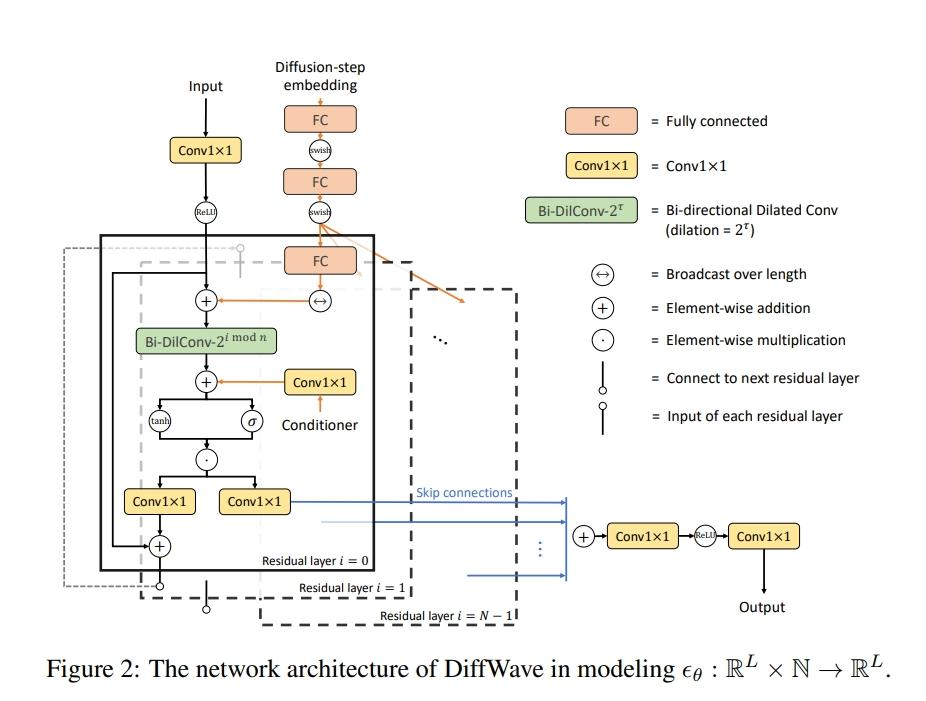
\includegraphics[width=\textwidth]
    {figures/part2_a/2.jpeg}
    \caption{Architecture du réseau de neurones DiffWave.
    Source : Kong et al., \textit{DiffWave: A Versatile Diffusion
    Model for Audio Synthesis}, ICLR 2021, Figure 2.}
    \label{fig:diffwave_architecture}
\end{figure}

\subsection{Applications et entrées/sorties du modèle}

DiffWave est conçu pour plusieurs tâches de génération de formes
d'onde audio. Les informations fournies au modèle dépendent de
l'application.

\subsubsection{Neural vocoding conditionné par un spectrogramme Mel}

Le \textit{neural vocoding} consiste à transformer une représentation
spectrale du signal vocal en une forme d'onde audio.

Dans cette application, DiffWave utilise un spectrogramme Mel comme
information de conditionnement locale. Ce spectrogramme est
généralement produit par un modèle de synthèse vocale
(\textit{text-to-spectrogram}).

Le spectrogramme Mel est suréchantillonné afin d'avoir la même
longueur temporelle que la forme d'onde. Il est ensuite injecté
dans les couches résiduelles du réseau.

\textbf{Entrées :}
\begin{itemize}
    \item un signal initial bruité $x_T$, échantillonné à partir
    d'une distribution gaussienne ;
    \item un spectrogramme Mel servant de conditionnement local.
\end{itemize}

\textbf{Sortie :}
\begin{itemize}
    \item une forme d'onde audio reconstruite correspondant
    au spectrogramme Mel fourni.
\end{itemize}

Cette application permet notamment de produire un signal vocal
à partir de caractéristiques spectrales, sans générer les
échantillons audio de manière autorégressive.

\subsubsection{Génération conditionnelle par classe}

Dans cette application, le modèle génère un signal audio en
fonction d'une étiquette globale, par exemple un identifiant
de locuteur (\textit{speaker ID}) ou un identifiant de mot
(\textit{word ID}).

L'étiquette est transformée en un vecteur d'embedding appris,
qui est ensuite injecté dans les différentes couches résiduelles
du réseau.

\textbf{Entrées :}
\begin{itemize}
    \item un bruit initial $x_T$ ;
    \item une étiquette de classe, de locuteur ou de mot.
\end{itemize}

\textbf{Sortie :}
\begin{itemize}
    \item une forme d'onde audio correspondant à la classe
    ou à l'identité spécifiée.
\end{itemize}

Le conditionnement permet ainsi de contrôler certaines
caractéristiques globales du signal généré.

\subsubsection{Génération audio inconditionnelle}

Dans le cas de la génération inconditionnelle, DiffWave ne reçoit
aucune information externe de conditionnement.

Le modèle apprend directement la distribution des formes d'onde
présentes dans les données d'entraînement. Il génère ensuite
de nouveaux signaux audio à partir d'un bruit gaussien.

\textbf{Entrée :}
\begin{itemize}
    \item un bruit initial $x_T$ échantillonné selon une
    distribution gaussienne standard.
\end{itemize}

\textbf{Sortie :}
\begin{itemize}
    \item une forme d'onde audio générée sans conditionnement
    externe.
\end{itemize}

Cette application est particulièrement intéressante car le
modèle doit apprendre les caractéristiques globales du signal
audio sans disposer d'un spectrogramme ou d'une étiquette
pour guider la génération.

\subsubsection{Résumé des applications}

Le Tableau~\ref{tab:diffwave_applications} résume les principales
applications présentées dans l'article original.

\begin{table}[htbp]
    \centering
    \caption{Applications de DiffWave et leurs entrées/sorties.}
    \label{tab:diffwave_applications}
    \begin{tabular}{|p{3.2cm}|p{5cm}|p{5cm}|}
        \hline
        \textbf{Application} &
        \textbf{Entrées} &
        \textbf{Sorties} \\
        \hline
        Neural vocoding &
        Bruit gaussien initial et spectrogramme Mel &
        Forme d'onde audio correspondant au spectrogramme Mel \\
        \hline
        Génération conditionnelle &
        Bruit gaussien initial et étiquette de classe ou de locuteur &
        Forme d'onde correspondant à la classe spécifiée \\
        \hline
        Génération inconditionnelle &
        Bruit gaussien initial uniquement &
        Nouvelle forme d'onde audio générée sans conditionnement \\
        \hline
    \end{tabular}
\end{table}

\subsection{Principe des modèles de diffusion}

Les modèles de diffusion sont des modèles génératifs qui apprennent
à transformer progressivement une distribution simple, généralement
une distribution gaussienne, en une distribution complexe correspondant
aux données réelles.

DiffWave utilise deux processus complémentaires :
\begin{itemize}
    \item le processus direct de diffusion
    (\textit{forward diffusion process}) ;
    \item le processus inverse de débruitage
    (\textit{reverse diffusion process}).
\end{itemize}

\subsubsection{Processus direct : ajout progressif du bruit}

On considère un signal audio original noté $x_0$.
Le processus direct consiste à ajouter progressivement du bruit
gaussien au signal pendant $T$ étapes.

La transition entre deux étapes successives est définie par :

\begin{equation}
q(x_t \mid x_{t-1}) =
\mathcal{N}
\left(
x_t ;
\sqrt{1-\beta_t}\,x_{t-1},
\beta_t I
\right)
\end{equation}

où :
\begin{itemize}
    \item $x_{t-1}$ représente le signal à l'étape précédente ;
    \item $x_t$ représente le signal après ajout de bruit ;
    \item $\beta_t$ est un paramètre contrôlant la quantité
    de bruit ajoutée ;
    \item $I$ est la matrice identité.
\end{itemize}

On définit également :

\begin{equation}
\alpha_t = 1-\beta_t
\end{equation}

et :

\begin{equation}
\overline{\alpha}_t =
\prod_{s=1}^{t}\alpha_s
\end{equation}

Grâce à cette formulation, le signal bruité à une étape quelconque
peut être obtenu directement à partir du signal original :

\begin{equation}
x_t =
\sqrt{\overline{\alpha}_t}\,x_0
+
\sqrt{1-\overline{\alpha}_t}\,\epsilon
\end{equation}

avec :

\begin{equation}
\epsilon \sim \mathcal{N}(0,I)
\end{equation}

Lorsque le nombre d'étapes augmente, la contribution du signal
original diminue progressivement et le signal devient de plus
en plus proche d'un bruit gaussien.

\subsubsection{Processus inverse : reconstruction du signal}

Le processus inverse consiste à partir d'un bruit gaussien
$x_T$ et à éliminer progressivement le bruit afin de reconstruire
un signal audio cohérent.

Le signal initial est échantillonné selon :

\begin{equation}
x_T \sim \mathcal{N}(0,I)
\end{equation}

Le réseau de neurones apprend à estimer le bruit présent à
chaque étape. Cette estimation est notée :

\begin{equation}
\epsilon_\theta(x_t,t)
\end{equation}

La moyenne de la distribution de transition inverse est
paramétrée par :

\begin{equation}
\mu_\theta(x_t,t)
=
\frac{1}{\sqrt{\alpha_t}}
\left(
x_t -
\frac{\beta_t}
{\sqrt{1-\overline{\alpha}_t}}
\epsilon_\theta(x_t,t)
\right)
\end{equation}

Le processus inverse est alors défini par :

\begin{equation}
p_\theta(x_{t-1}\mid x_t)
=
\mathcal{N}
\left(
x_{t-1};
\mu_\theta(x_t,t),
\widetilde{\beta}_t I
\right)
\end{equation}

où :

\begin{equation}
\widetilde{\beta}_t
=
\frac{1-\overline{\alpha}_{t-1}}
{1-\overline{\alpha}_t}
\beta_t
\end{equation}

Le processus est répété pour $t=T,T-1,\ldots,1$ jusqu'à obtenir
le signal final $x_0$.

La Figure~\ref{fig:diffwave_diffusion} illustre les deux
processus : l'ajout progressif de bruit et la reconstruction
du signal audio.

\begin{figure}[htbp]
    \centering
    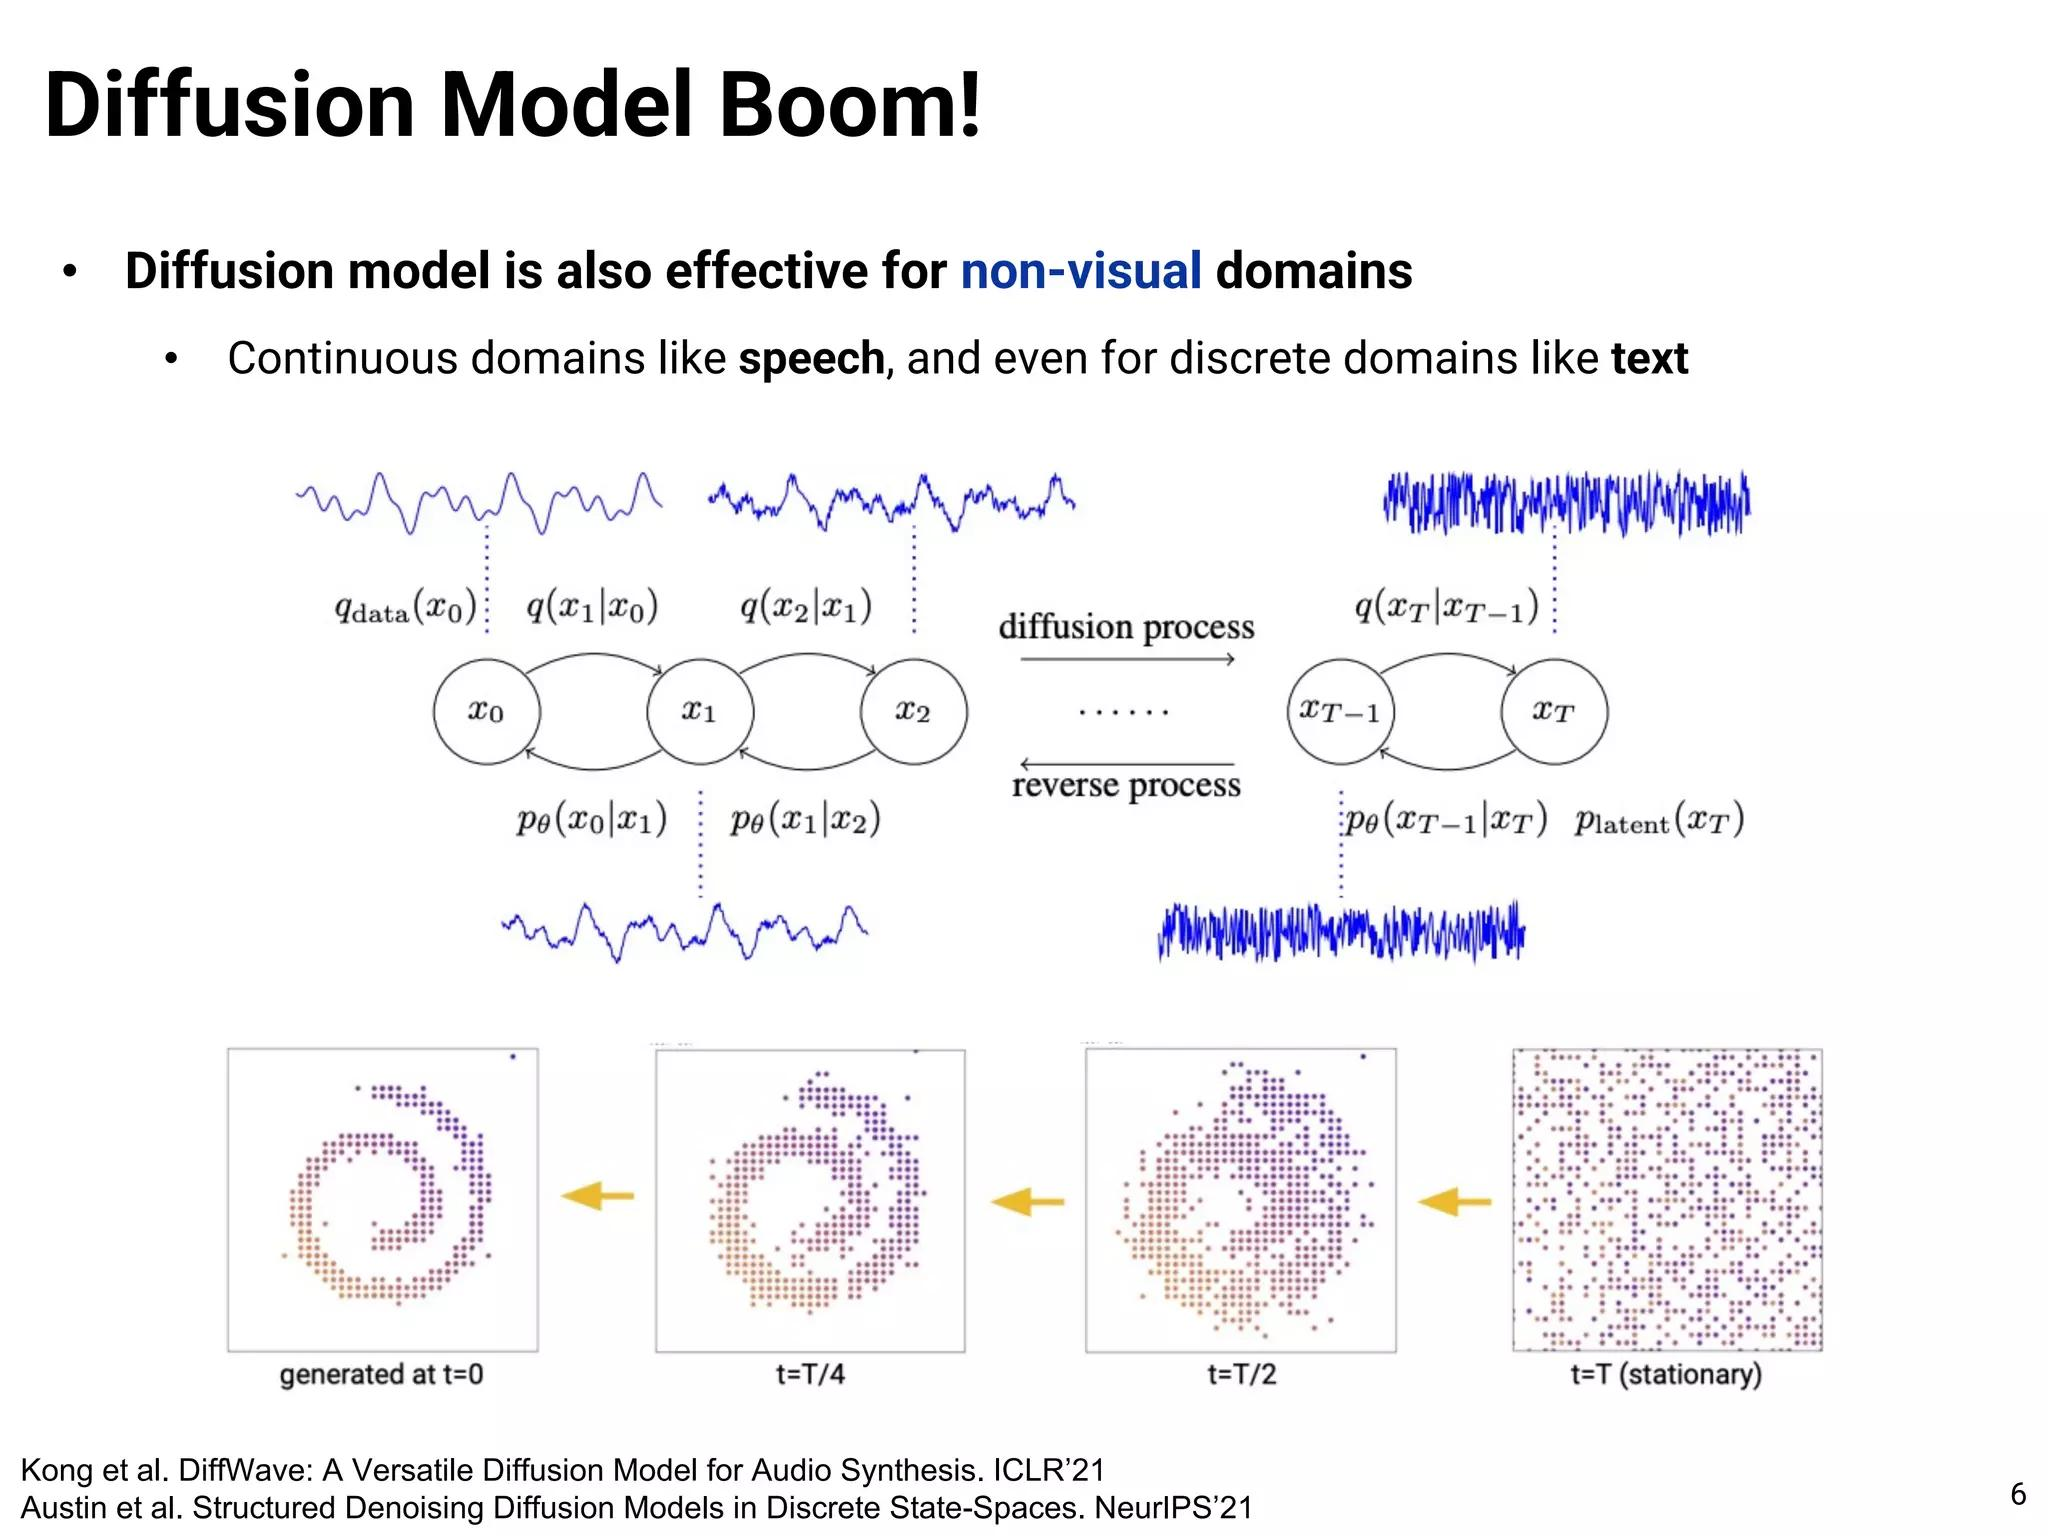
\includegraphics[width=0.90\textwidth]
    {figures/part2_a/1.jpeg}
    \caption{Processus direct de diffusion et processus inverse
    de reconstruction dans un modèle de diffusion.
    Source : Kong et al., \textit{DiffWave: A Versatile Diffusion
    Model for Audio Synthesis}, ICLR 2021, Figure 1.}
    \label{fig:diffwave_diffusion}
\end{figure}

\subsection{Principe d'apprentissage du réseau}

L'objectif de l'apprentissage est de permettre au réseau de
prédire correctement le bruit gaussien ajouté au signal original.

Pendant l'entraînement, on effectue les opérations suivantes :
\begin{enumerate}
    \item On sélectionne un signal audio original $x_0$ dans
    la base de données.
    \item On génère un bruit gaussien
    $\epsilon \sim \mathcal{N}(0,I)$.
    \item On choisit aléatoirement une étape de diffusion $t$.
    \item On construit le signal bruité $x_t$ à partir de
    $x_0$ et de $\epsilon$.
    \item On fournit $x_t$ et $t$ au réseau, ainsi que
    l'information de conditionnement lorsqu'elle est utilisée.
    \item Le réseau prédit le bruit
    $\epsilon_\theta(x_t,t,c)$.
    \item On compare le bruit réel au bruit estimé et on
    ajuste les paramètres du réseau.
\end{enumerate}

Pour les applications conditionnelles, $c$ représente l'information
de conditionnement, par exemple le spectrogramme Mel ou une
étiquette globale.

La fonction de coût utilisée est une erreur quadratique moyenne
entre le bruit réel et le bruit estimé :

\begin{equation}
\mathcal{L}(\theta)
=
\mathbb{E}_{x_0,\epsilon,t}
\left[
\left\|
\epsilon -
\epsilon_\theta
\left(
\sqrt{\overline{\alpha}_t}x_0
+
\sqrt{1-\overline{\alpha}_t}\epsilon,
t,c
\right)
\right\|_2^2
\right]
\end{equation}

Cette fonction de coût permet au réseau d'apprendre à identifier
le bruit présent dans des signaux audio à différents niveaux
de corruption.

\subsection{Notion de conditionnement dans DiffWave}

Le conditionnement (\textit{conditioning}) consiste à fournir
au modèle une information supplémentaire afin de guider la
génération du signal audio.

L'article distingue deux formes principales de conditionnement.

\subsubsection{Conditionnement local}

Le conditionnement local est une information qui varie dans
le temps et qui est alignée avec la forme d'onde.

Dans l'application de neural vocoding, cette information
correspond au spectrogramme Mel.

Le spectrogramme est d'abord suréchantillonné afin d'obtenir
la même longueur temporelle que le signal audio. Il est ensuite
transformé par des convolutions $1\times1$ et injecté dans
les couches résiduelles du réseau.

Il permet de guider la génération en imposant les caractéristiques
spectrales et temporelles du signal à reconstruire.

\subsubsection{Conditionnement global}

Le conditionnement global représente une information qui
caractérise l'ensemble du signal, sans varier à chaque instant.

Il peut s'agir, par exemple :
\begin{itemize}
    \item d'un identifiant de locuteur ;
    \item d'un identifiant de mot ;
    \item d'une étiquette représentant une classe audio.
\end{itemize}

Cette information est transformée en un vecteur d'embedding
appris, puis injectée dans les couches résiduelles.

Elle permet de contrôler les caractéristiques globales du
signal généré.

\subsubsection{Génération sans conditionnement}

Dans le cas de la génération inconditionnelle, aucune information
externe n'est fournie au réseau.

Le modèle reçoit uniquement le signal bruité et l'étape de
diffusion. Il doit donc apprendre à générer des formes d'onde
cohérentes à partir de la distribution des données d'entraînement.

\subsection{Différences entre DiffWave et WaveNet}

WaveNet est un modèle génératif audio basé sur une architecture
autorégressive. Il génère les échantillons audio successivement,
en utilisant les échantillons précédemment générés pour prédire
le suivant.

DiffWave adopte une approche différente : il utilise un modèle
de diffusion non autorégressif basé sur des convolutions
dilatées bidirectionnelles.

Les principales différences sont résumées dans le tableau
suivant.

\begin{table}[htbp]
    \centering
    \caption{Comparaison entre DiffWave et WaveNet.}
    \label{tab:diffwave_wavenet}
    \begin{tabular}{|p{3cm}|p{5cm}|p{5cm}|}
        \hline
        \textbf{Critère} &
        \textbf{WaveNet} &
        \textbf{DiffWave} \\
        \hline
        Type de modèle &
        Autorégressif &
        Non autorégressif \\
        \hline
        Principe de génération &
        Génération séquentielle des échantillons &
        Débruitage itératif d'une forme d'onde complète \\
        \hline
        Architecture &
        Convolutions causales dilatées &
        Convolutions dilatées bidirectionnelles \\
        \hline
        Dépendance temporelle &
        Chaque échantillon dépend des précédents &
        Le réseau exploite le contexte temporel dans
        les deux directions \\
        \hline
        Parallélisation &
        Limitée pendant la génération autorégressive &
        Calcul parallèle sur les échantillons à chaque
        étape de diffusion \\
        \hline
        Génération &
        Un échantillon à la fois &
        Plusieurs étapes successives de débruitage \\
        \hline
    \end{tabular}
\end{table}

DiffWave présente ainsi un avantage important en matière de
parallélisation, car il ne nécessite pas de générer chaque
échantillon audio individuellement.

Cependant, il faut noter que son processus de génération
reste itératif : plusieurs étapes de diffusion inverse sont
nécessaires pour obtenir le signal final.

Dans les expériences présentées par les auteurs, DiffWave
atteint une qualité vocale comparable à celle de WaveNet,
avec des scores MOS respectifs de 4,43 et 4,44. Les auteurs
rapportent également une génération beaucoup plus rapide
dans leur configuration expérimentale.

\subsection{Conclusion}

DiffWave est un modèle génératif audio basé sur les processus
de diffusion probabilistes. Il transforme progressivement
un bruit gaussien en une forme d'onde audio grâce à un réseau
de neurones qui apprend à prédire le bruit à chaque étape.

Son architecture non autorégressive, construite autour de
convolutions dilatées bidirectionnelles, lui permet de traiter
les échantillons audio en parallèle au sein de chaque étape
de débruitage.

Les trois applications principales étudiées dans l'article
sont le neural vocoding conditionné par un spectrogramme Mel,
la génération conditionnelle par classe et la génération
inconditionnelle.

Grâce à la possibilité d'utiliser des informations de
conditionnement locales ou globales, DiffWave constitue
une architecture flexible pour la synthèse de formes d'onde
audio.
